\documentclass[11pt,letterpaper]{article}
\usepackage[utf8]{inputenc} %Codificacion del texto (ISO Latin1 encoding)

\usepackage{fancyhdr} %Permite acomodar a tu gusto la parte de arriba y
% abajo del documento
\usepackage[spanish]{babel} %Permite definir el idioma del dcumento
\usepackage{graphicx} %Permite exportar imagenes en formato eps
\usepackage{url} %Tipo de fuente para correos y paginas
\usepackage{pgf}
\usepackage{fleqn}
\usepackage{amssymb}
\usepackage{fancyvrb}
\usepackage{sectsty}
\usepackage{makeidx}
\usepackage{colortbl} %Permite colocar colores a las tablas
\usepackage{booktabs}
%%%%%%%%%%
%Margenes%
%%%%%%%%%%
\parskip 1mm %Espacio entre parrafos

\setlength{\topmargin}{0pt}

\oddsidemargin	0.5cm  % Ancho Letter 21,59cm
\evensidemargin 0.5cm  % Alto  Letter 27,81cm
\textwidth	15.5cm
\textheight	21.0cm
\headsep	4 mm
\parindent	0.5cm
%%%%%%%%%%%%%%%%%%%%%%
%Estilo del documento%
%%%%%%%%%%%%%%%%%%%%%%
\pagestyle{fancyplain}

%%%%%%%%%%%%%%%%%%%%%%%%%%%%%%%%%%%%%%%%%%%
%Fancyheadings. Top y Bottom del documento%
%%%%%%%%%%%%%%%%%%%%%%%%%%%%%%%%%%%%%%%%%%%
% Recuerde que en este documento la portada del documento no posee
% numeracion, pero de igual manera llamaremos a esa primera pagina la numero
% 1, y la que viene la dos. Esto es para tener una idea de las que
% llamaremos pares e impares
\lhead{Fundamentos de Ingeniería de Software} %Parte superior izquierda
\rhead{\bf \it Tarea 1} %Parte superior derecha
\lfoot{\it Septiembre 2008} %Parte inferior izquierda. \thepage indica
% el numero de pagina
\cfoot{} %Parte inferior central
\rfoot{\bf \thepage} %Parte inferior derecha
\renewcommand{\footrulewidth}{0.4pt} %Linea de separacion inferior

% Challa

\newtheorem{theorem}{Theorem}
\newtheorem{acknowledgement}[theorem]{Acknowledgement}
\newtheorem{algorithm}[theorem]{Algorithm}
\newtheorem{axiom}[theorem]{Axiom}
\newtheorem{case}[theorem]{Case}
\newtheorem{claim}[theorem]{Claim}
\newtheorem{conclusion}[theorem]{Conclusion}
\newtheorem{condition}[theorem]{Condition}
\newtheorem{conjecture}[theorem]{Conjecture}
\newtheorem{corollary}[theorem]{Corollary}
\newtheorem{criterion}[theorem]{Criterion}
\newtheorem{definition}[theorem]{Definition}
\newtheorem{example}[theorem]{Example}
\newtheorem{exercise}[theorem]{Exercise}
\newtheorem{lemma}[theorem]{Lemma}
\newtheorem{notation}[theorem]{Notation}
\newtheorem{problem}[theorem]{Problem}
\newtheorem{proposition}[theorem]{Proposition}
\newtheorem{remark}[theorem]{Remark}
\newtheorem{solution}[theorem]{Solution}
\newtheorem{summary}[theorem]{Summary}
\newenvironment{proof}[1][Proof]{\noindent\textbf{#1.} }{\ \rule{0.5em}{0.5em}}

\newcommand{\primaria}[1]{
	\textbf{\underline{#1}}
}

\newcommand{\foranea}[1]{
	\textbf{\textsl{#1}}
}

\newcommand{\primyfor}[1]{
	\underline{\foranea{#1}}
}

\makeatletter
\newcommand\subsubsubsection{\@startsection {paragraph}{1}{\z@}%
                                   {-3.5ex \@plus -1ex \@minus -.2ex}%
                                   {1.5ex \@plus.2ex}%
                                   {\normalfont\bfseries}}
\newcommand\subsubsubsubsection{\@startsection {subparagraph}{1}{\z@}%
                                   {-3.5ex \@plus -1ex \@minus -.2ex}%
                                   {1.5ex \@plus.2ex}%
                                   {\normalfont\bfseries}}


\makeatother

%\makeindex
%%%%%%%%%%%%%%%%%%%%%%%%%%%%%%%%%%%%%%%%%%%%%%%%%%%%%%%%%%%%%%%%%%%
%%%%%%%%%%%%%%%%%%%% Aqui empieza el documento %%%%%%%%%%%%%%%%%%%%
%%%%%%%%%%%%%%%%%%%%%%%%%%%%%%%%%%%%%%%%%%%%%%%%%%%%%%%%%%%%%%%%%%%

\begin{document}

%%%%%%%%%%%%%%%%%%%%%%%%%%
%Definicion de la portada%
%%%%%%%%%%%%%%%%%%%%%%%%%%
\begin{titlepage}
    \begin{center}
	\begin{tabular}{ccc}
	    %\epsfig{file=escudo-utfsm.eps, height=1.6cm}
	      
\includegraphics[height=1.6cm]{images/logoUTFSM}
	    & %Escudo de la Universidad Santa Maria
	    \hspace{0.2cm}
	    \begin{tabular}{c}
		Universidad Técnica Federico Santa María \\ \hline
		\hspace{8.0cm}
		\vspace{1.2cm}
	    \end{tabular}
	    \hspace{0.2cm}
	    &
	   % \epsfig{file=logo_DI.eps, height=1.6cm} %Logo del DI
            
\includegraphics[height=1.6cm]{images/logoDI}
	\end{tabular}

	\vspace{2.5cm}
	%Titulo del Documento
	    \begin{tabular}{c}
		\Huge{\textbf{Tarea 2}}\\\\\\\\\\\\\\
		\LARGE{\textbf{``Sistema de Gesti\'on de Clientes VIP''}}\\\\
		\LARGE{\sc{Fundamentos de Ingenier\'ia}}\\
		\LARGE{\sc{de Software}}
	    \end{tabular}

	\vspace{2.5cm}
%	\begin{tabular}{c}
	\begin{center}
%	     \pgfimage[height=1.8cm]{images/now}
	%    \Huge{\emph{Now!}}
%	\end{tabular}
	\end{center}
	
        \vspace{1.5cm}

	%Nombre del (o los) autor(es)
	\begin{tabular}{lr}
            \begin{tabular}{c}
	        \large{Rodrigo Fern\'andez - 2673002-3}\\
		\large{\url{rfernand@inf.utfsm.cl}}
	    \end{tabular}
	&
	   \begin{tabular}{c}
         	\large{Cristi\'an Maureira - 2673030-9}\\ 
		\large{\url{cmaureir@inf.utfsm.cl}}
	   \end{tabular}
	\end{tabular}
        \vspace{3.5cm}\\
	%Fecha
		\large{\sc{Valpara\'iso, Octubre 2008.}}
    \end{center}
\end{titlepage}


\section{Diagrama de Casos de Uso}
\label{sec:diagrama}
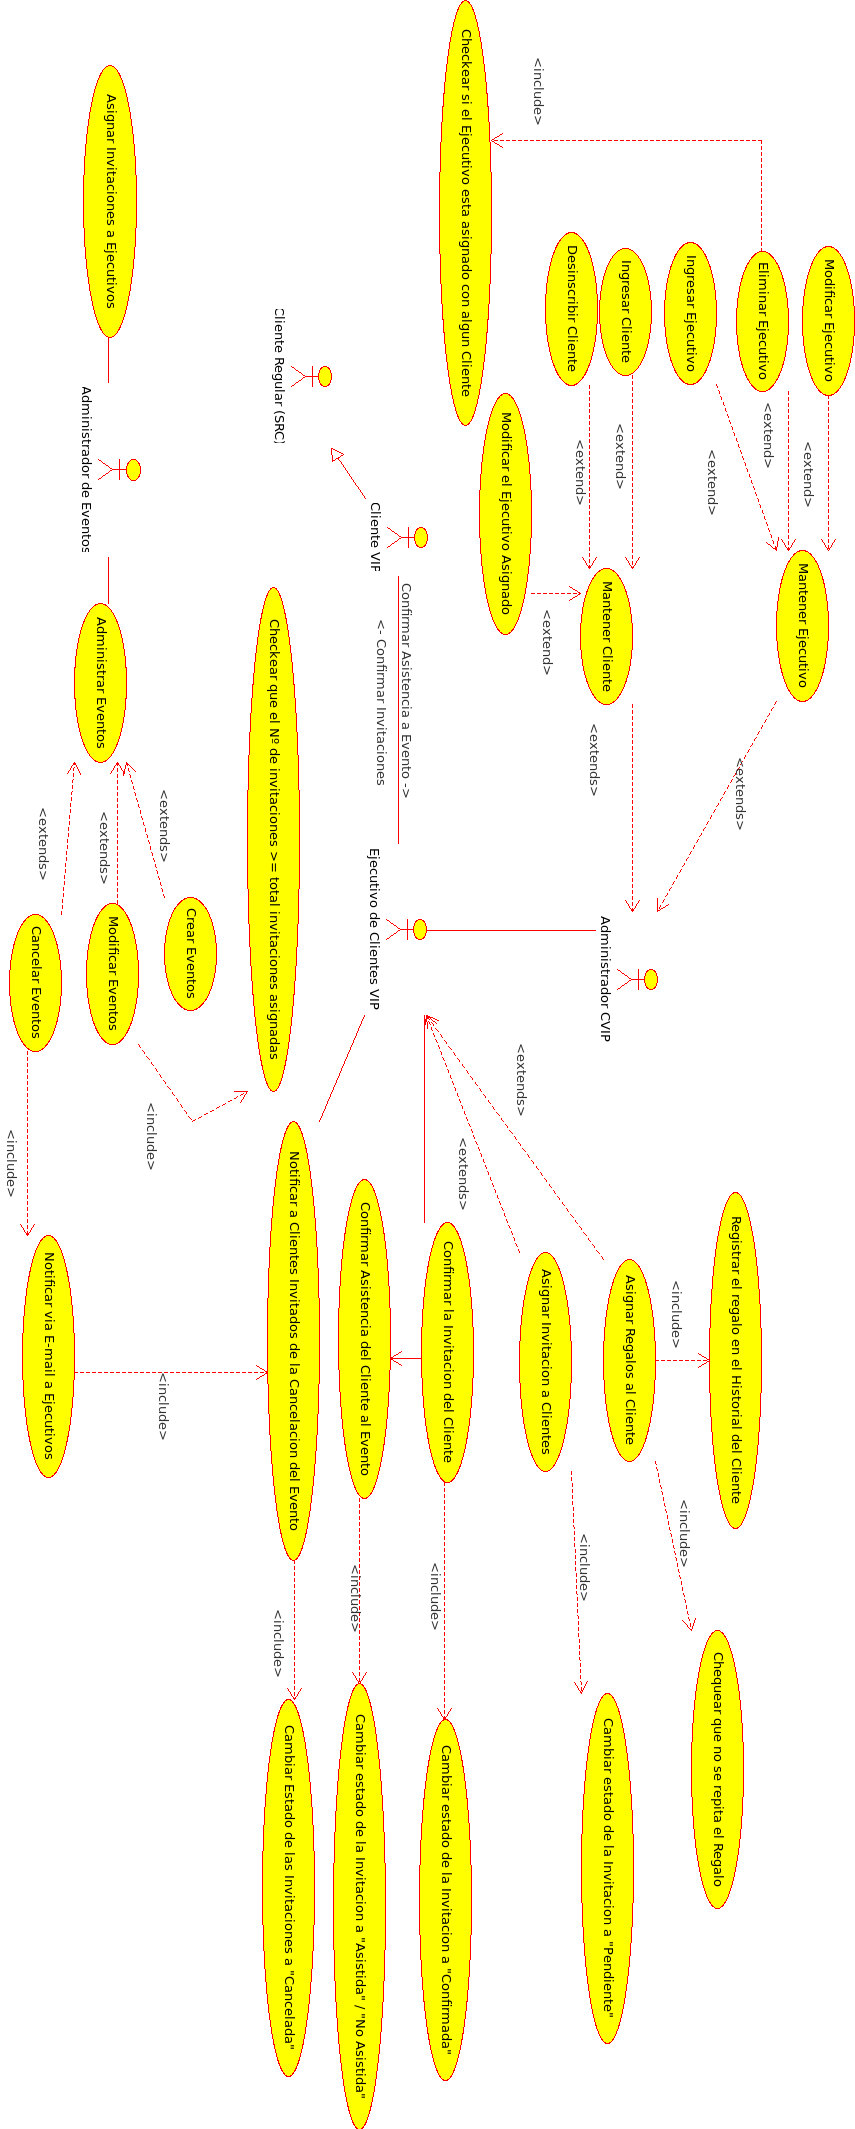
\includegraphics[height=19.5cm,width=11cm]{images/casoDeUso}




\subsection{Lista de Actores}
\label{sec:actores}
\begin{itemize}
	\item Cliente VIP
	\item Ejecutivo de Clientes VIP
	\item Administrador de Eventos
	\item Sistema de Gestion de Clientes VIP (CVIP)
	\item Sitema de Clientes Regulares (SCR)
\end{itemize}


\subsection{Resumen de Casos de Uso}
\label{sec:casosdeuso}
\begin{enumerate}
	\item Cliente VIP
	\begin{itemize}
		\item Responder solicitudes de confirmaci\'on de invitaciones.
		\item Responder solicitudos de confirmaci\'on de aistencias a eventos.
	\end{itemize}
	\item Ejecutivo del Cliente
	\begin{itemize}	
		\item Asignar invitaci\'on/es a Clientes VIP.
		\item Cambiar el estado de la invitaci\'on dependiendo de la ocasion.
		\item Notificar sobre Cancelaciones de Eventos a los Clientes.
		\item Solicitar confirmacion de invitaciones / asitencias a los clientes VIP sobre cada evento.
		\item Ver los Clientes VIP de cumplea\~nos dentro de los pr\'oximos 5 dias.
		\item Seleccionar Regalo de la Lista de Regalos.
		\item Asignar Regalo a Clientes VIP sin que se repita.

	\end{itemize}
	\item Administrador de Eventos
	\begin{itemize}
		\item Realizar sobre Evento las operaciones de:
		\begin{itemize}
			\item Crear 
			\item Modificar
			\item Cancelar
			\item Asignar invitaciones del evento a los Ejecutivos
		\end{itemize}
		\item Enviar Correo a los Ejecutivos si un evento de cancela 
	\end{itemize}
	\item Administrador del CVIP
	\begin{itemize}
		\item Realizar sobre Regalo las operaciones de:
		\begin{itemize}
			\item Ingresar
			\item Modificar
			\item Crear
		\end{itemize}
		\item Realizar sobre Ejecutivo de Clientes VIP las operaciones de:
		\begin{itemize}
			\item Ingresar
			\item Modificar Datos
			\item Eliminar
		\end{itemize}
		\item Realizar sobre los Clientes VIP las operaciones de:
		\begin{itemize}
			\item Ingresar
			\item Inscribir un Cliente del SCR como VIP
			\item Asignar Ejecutivo
			\item Desincribir
			\item Modificar Ejecutivo Asignado
		\end{itemize}
	\end{itemize}
\end{enumerate}


\subsection{Relaciones}
\label{sec:relaciones_casos}
Las relaciones se pueden ver en el diagrama de los casos de Uso.


\section{Modelo de Dominio}
\label{sec:mdominio}
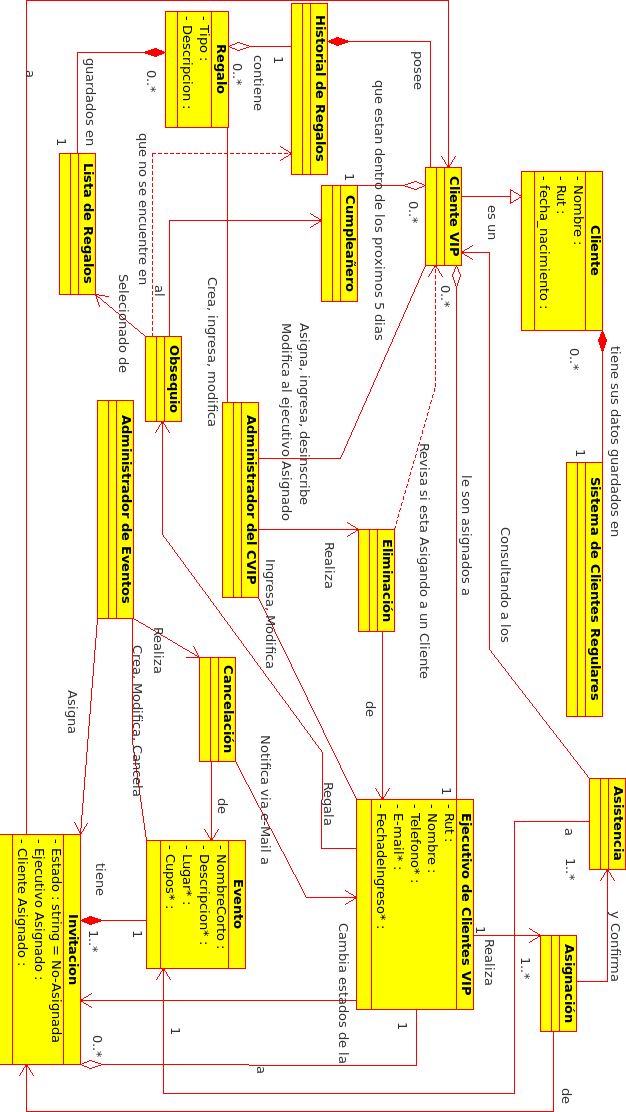
\includegraphics[height=19.5cm,width=11cm]{images/modeloEstatico}


\subsection{Entidades del Dominio}
\label{sec:entidades}
\begin{itemize}
	\item Cliente
	\item Clientes VIP
	\item Sistema de Clientes Regulares
	\item Ejecutivo de Clientes VIP
	\item Administrador de Eventos
	\item Invitaci\'on
	\item Evento
	\item Cumplea\~nero
	\item Regalo
	\item Obsequio
	\item Lista de Regalos
	\item Historial de Regalos
	\item Asistencia
	\item Asignaci\'on
	\item Eliminaci\'on
\end{itemize}


\subsection{Atributos de las Entidades}
\label{sec:atributos}
Los atributos pueden verse claramente en el diagrama, y por motivos de tiempo y perdida de m\'as \'arboles para la producci\'on del papel, no seran expuestos en el informe.



\subsection{Relaciones}
\label{sec:relaciones_ent}
Al igual que los atributos, las relaciones se pueden ver en el diagrama de entidades.


\subsection{Supuestos}
\label{sec:supuestos}
\begin{itemize}
	\item Consideramos que seria bueno que el Administrador de Eventos sea identificable para poder reconocer a posterioridad que administrador de Eventos realizo los mejores eventos, o cometio errores al realizar algo.
	\item Se considero que el curso normal de los eventos, pueden haber diferentes Adminsitradores del Sistema trabajando paralelamente, por lo que habia que validar los datos para evitar inconsistencias en la base de datos.
	\item Se adapt\'o el diagrama de casos de uso segun la pauta dada en la tarea.
	\item Se considero que seg\'un el texto, el que manten\'ia los eventos era el Administrador de Eventos y no el Administrador del Sistema.
\end{itemize}


\subsection{Criterios de Modelamiento}
\label{sec:criterios}
\begin{itemize}
	\item Casi todas las condiciones para desarrollar algun proceso, fueron plasmadas con un ``include'' en los casos de uso para que se verificara la
		condicion antes de realizar el acto.
	\item Se establecieron los diferentes casos de uso en sectores diferentes del diagrama para notar el conjunto de funcionalidades de cada
		requerimiento
	\item En el modelo estatico, se utilizaron flechas direccionales para facilitar la lectura visual de las relaciones, y se agruparon las funcionalidades como ingrsar, modificar, inscribir, etc. para poder simplificar el diagrama. Tambien, se crearon clases que pueden sonar que repiten informacion (como obsequio y regalo), pero que se identifican con procesos diferentes, relacionandose con diferentes entidades y por ende, fueron identificados como entidades aparte.
\end{itemize}



\subsection{Descripción Herramienta Utilizada}
\label{sec:umbrello}
\begin{center}
	
\includegraphics[height=1.5cm]{images/umbrello}\\
\end{center}
\textbf{Umbrello} es una herramienta libre para crear y editar diagramas UML, que ayuda en el proceso del desarrollo de software. Fue desarrollada por Paul Hensgen, y está diseñado principalmente para KDE, aunque funciona en otros entornos de escritorio.\\

Umbrello maneja gran parte de los diagramas estándar UML pudiendo crearlos, además de manualmente, importándolos a partir de código en C++, Java, Python, IDL, Pascal/Delphi, Ada, o también Perl (haciendo uso de una aplicación externa). Así mismo, permite crear un diagrama y generar el código automáticamente en los lenguajes antes citados, entre otros. El formato de fichero que utiliza está basado en XMI.\\

También permite la distribución de los modelos exportándolos en los formatos DocBook y XHTML, lo que facilita los proyectos colaborativos donde los desarrolladores no tienen acceso directo a Umbrello o donde los modelos van a ser publicados vía web.Umbrello se distribuye en el módulo kdesdk de KDE.\\

\textbf{Web:} http://uml.sourceforge.net/



\end{document}
